\ifx\atempxetex\usewhat
\XeTeXinputencoding "utf-8"
\fi
\defaultfont

\chapter{文件I/O}

本章介绍了文件读写的基本要素。这些操作构成了Unix系统的核心。第三章将介绍基于C标准库的标准I/O,而第四章继续讨论了更高级和专门化的I/O接口。第七章以文件和目录操作为主题结束了整个文件I/O部分的讨论。

在对文件进行读写操作前,需要先打开该文件。内核为每个进程维护一个打开文件的列表,该表被称为文件表(file table)。该表由一些叫做文件描述符(file descriptors)(常缩写作 fds)的非负整数进行索引。列表中的每项均包含一个打开文件的信息,其中包括一个指向文件备份inode内存拷贝的指针和元数据(例如文件位置和访问模式等)。用户空间和内核空间都把文件描述符作为每个进程的唯一cookies。打开一个文件返回一个文件描述符,而接下来的操作(读写等等)则把文件描述符作为基本参数。

子进程默认会获得一份父进程的文件表拷贝。 其中打开文件列表、访问模式,当前文件位置等信息都是一致的。进程中文件表的变化(例如子进程关闭文件)也不会影响其他进程的文件表。然而,就如你将在第五章了解到的,可以让子进程和父进程共享后者的文件表(就像线程那样)。

文件描述符由C语言的int类型表示。不使用fd\_t这个特殊类型来表示,虽然看上去有些古怪,但实际上,这是沿袭了Unix的传统。每个 Linux进程有一个打开文件数的上限。 文件描述符从0开始,直到比上限小1。默认的上限是1,024,但最多可以将该值设定为1,048,576。 负数不是合法的文件描述符,所以 -1 常常被用来表示一个函数不能返回合法文件描述符的错误。

每个进程按照惯例会至少有三个打开的文件描述符:0,1和2,除非进程显式的关闭它们。文件描述符0是标准输入(stdin),文件描述符1是标准输出(stdout),而文件描述符2是标准错误(stderr)。 C标准库提供了预处理器宏:STDIN\_FILENO,STDOUT\_FILENO和STDERR\_FILENO宏,以取代对以上整数的直接引用。

需要注意的是,文件描述符不仅仅用于普通文件的访问,也用于访问设备文件、管道、目录以及快速用户空间锁、FIFOs和套接字。遵循一切皆文件的理念,任何你能读写的东西都可以用文件描述符来访问。 

\section{打开文件}
最基本的访问文件的方法是使用read()和write()系统调用。 在一个文件能被访问之前,必须通过open()或者creat()系统调用打开它。 一旦使用完毕,就应该用close()系统调用来关闭文件。 

\subsection{open()系统调用}
通过open()系统调用来打开一个文件并获得一个文件描述符。 
\begin{lstlisting}
  #include <sys/types.h>
  #include <sys/stat.h>
  #include <fcntl.h>

  int open (const char *name, int flags);
  int open (const char *name, int flags, mode_t mode);
\end{lstlisting}
open()系统调用将路径名name给出的文件与一个成功返回的文件描述符相关联,文件位置指针被设定为零,而文件则根据flags给出的标志位打开。
\subsubsection{open()的flags参数}
flags 参数必须是以下之一:O\_RDONLY,O\_WRONLY或者O\_RDWR。 这些参数各自指定要用只读,只写还是读写模式打开文件。

举例来说,下面的代码以只读方式打开文件 /home/kidd/madagascar 。 
\begin{lstlisting}
  int fd;

  fd = open (``/home/kidd/madagascar'', O_RDONLY);
  if (fd==-1)
      /* error */
\end{lstlisting}
以只写模式打开的文件不能被读取,反之亦然。进程必须要有足够的权限才能调用open()系统调用对文件进行访问。

flags参数可以和以下一个或多个值进行按位或运算,用以修改打开文件请求的行为。
\begin{eqlist*}
\item [O\_APPEND]
文件将以追加模式下打开。 就是说,在每次写操作之前,文件位置指针将被置于文件末尾。 即使在进程刚刚完成写操作并改变文件位置指针之后,如有另一进程开始写操作,情形也是如此。(参见本章后的“追加模式”) 
\item [O\_ASYNC]
当指定文件可写或者可读时产生一个信号(默认是 SIGIO)。 这个标志仅用于终端和套接字,不能用于普通文件。 
\item [O\_CREAT]
当name指定的文件不存在时,将由内核来创建。 如果文件已存在,本标志无效,除非给出了O\_EXCL标志。 
\item [O\_DIRECT]
打开文件用于直接I/O(参见本章后面的“直接I/O”)。 
\item [O\_DIRECTORY]
如果name不是一个目录,open()调用将会失败。这个标志用于在opendir()内部使用。 
\item [O\_EXCL]
和O\_CREAT一起给出的时候,如果由name给定的文件已经存在,则open()调用失败。 用来防止文件创建时出现竞争。 
\item [O\_LARGEFILE]
给定文件打开时将使用64位偏移量, 这样大于2G的文件也能被打开。 在64位架构中隐含是使用该参数来打开文件的。 
\item [O\_NOCTTY]
如果给出的name指向一个终端设备(也就是说,/dev/tty), 它将不会成为这个进程的控制终端, 即使该进程目前没有控制终端。 这个标志不大常用。 
\item [O\_NOFOLLOW]
如果name是一个符号链接, open()调用会失败。 通常,会解析该链接并且打开目标文件。 如果给出路径的其它部分是链接, 该调用仍可用。举例来说,如果name是/etc/ship/plank.txt,如果plank.txt是一个符号链接则该调用失败。然而,如果etc或者ship是符号链接,只要plank.txt不是,那么调用成功。 
\item [O\_NONBLOCK]
如果可以,文件将在非阻塞模式下打开。 open()调用不会,任何其它操作都不会使该进程在I/O中阻塞(sleep)。这种情况可能只用于FIFO。 
\item [O\_SYNC]
打开文件用于同步I/O。 在数据写到磁盘之前写操作不会完成;一般的读操作已是同步的,所以这个标志对读操作没有影响。 POSIX额外定义了O\_DSYNC和O\_RSYNC;在Linux上,这些标志与O\_SYNC同义。(参见本章后面的“O\_SYNC标志”。) 
\item [O\_TRUNC]
如果文件存在,且为普通文件,并允许写,将文件的长度截断为0。 对于FIFO或者终端设备,该参数被忽略。 在其它文件类型上则没有定义。 因为截断文件需要写权限,所以O\_TRUNC和O\_RDONLY同时使用也是没有定义的。\footnote[1]{译者注:O\_TRUNC | O\_RDONLY 在典型的Linux系统下(2.6内核+GCC4.2),结果将等同于只有O\_TRUNC。}
\end{eqlist*}

\begin{lstlisting}
  int fd;
 
  fd = open ("/home/teach/pearl", O_WRONLY | O_TRUNC);
  if (fd == -1)
      /* error */
\end{lstlisting}

\subsection{新文件所有者}
确定哪个用户拥有新建立文件是很简单的:文件所有者的用户id就是创建该文件的进程的有效用户id。决定所有用户组则稍麻烦些。 默认是将创建文件的进程的组id赋予该文件。这是System V的做法(Linux大部分系统行为以System V为模型),也是标准Linux的处理方法。

然而,麻烦点的是,BSD定义它自己的做法: 文件的组定为其上级目录的组id。这种做法在Linux上可通过挂载选项实现\footnote[1]{对应挂载选项bsdgroups或者sysvgroups。}——如果文件上级目录设置了设置组ID位(setgid),Linux的默认行为也将如此。尽管大多数Linux系统会采纳系统V的做法(新文件得到创建进程的组ID),而保留BSD做法(新文件得到上级目录组id)意味着那些真正需要关心的代码需使用chown()系统调用来手动设置组。

好在关注文件所有组的情况并不常见。 

\subsection{新文件权限}
前面给出的两种open()系统调用方式都是合法的。 除非创建了新文件,否则mode参数会被忽略;而当O\_CREAT给出时则需要。 如果你在使用O\_CREAT时忘记了提供mode参数,结果是未定义的,而且通常会很糟糕——所以千万别忘记!

当文件创建时,mode参数提供新建文件的权限。 系统并不在该次打开文件时检查权限,所以你可以进行相反的操作,例如设置文件为只读权限,但却在打开文件后进行写操作。

mode参数是常见的Unix权限位集合,像八进制数0644(所有者可以读写,其他人只能读)。从技术层面来讲,POSIX允许对特定实现指定具体的值,允许不同的Unix系统设置任何自己需要的位。为补偿权限位上的不可移植性,POSIX引入了一组可以进行按位或操作的常数,以满足对于mode参数的需求。 

\begin{eqlist*}
\item [S\_IRWXU]
所有者拥有读写和执行权限。 
\item [S\_IRUSR]
所有者拥有读权限。 
\item [S\_IWUSR]
所有者拥有写权限。 
\item [S\_IXUSR]
所有者拥有执行权限。 
\item [S\_IRWXG]
组拥有读写和执行权限。 
\item [S\_IRGRP]
组拥有读权限。 
\item [S\_IWGRP]
组拥有写权限。 
\item [S\_IXGRP]
组拥有执行权限。
\item [S\_IRWXO]
任何其他人都有读写和执行权限。 
\item [S\_IROTH]
任何其他人都有读权限。 
\item [S\_IWOTH]
任何其他人都有写权限。 
\item [S\_IXOTH]
任何其他人都有执行权限。 
\end{eqlist*}

实际上,最终写入磁盘的权限位还需让mode参数与用户文件创建的掩码(即umask)做按位与操作后来确定。通俗的说,umask中的位在和 open()给出的mode参数操作时要取反。 也就是,通常的umask 022将使mode参数0666变为0644(0666 \& $\sim$022)。对于系统程序员来说,在设置权限时不需要考虑umask——umask是允许用户对他的程序对新文件做权限限定时使用的。

举个例子,下面的代码对文件file进行写操作。如果文件不存在,且假定umask值为022,将建立权限值为0644的文件(即使mode参数指定为0664)。 如果已经存在,它的长度会被截短成0: 
\begin{lstlisting}
  int fd;
 
  fd = open (file, O_WRONLY | O_CREAT | O_TRUNC,
             S_IWUSR | S_IRUSR | S_IWGRP| S_IRGRP | S_IROTH);
  if (fd == -1)
     /* error */
\end{lstlisting}

\subsection{creat()函数}
O\_WRONLY | O\_CREAT | O\_TRUNC 组合经常被使用,以至于专门有个系统调用来实现。 

\begin{lstlisting}
  #include <sys/types.h>
  #include <sys/stat.h>
  #include <fcntl.h>

  int creat (const char *name, mode_t mode);
\end{lstlisting}
\par
\begin{wrapfigure}{l}{2.5cm}
  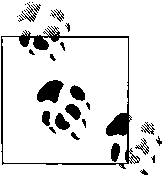
\includegraphics[width=2cm,clip]{paipai.png}
\end{wrapfigure}
\mbox{}\begin{flushleft}是的,这个函数名的确少个e。 Ken Thompson,Unix的创建者,曾开玩笑说漏掉这个字母是他设计Unix中最后悔的事情。\end{flushleft} 
\par
典型的creat()调用如下: 
\begin{lstlisting}
  int fd;
  fd = creat (file, 0644);
  if (fd == -1)
      /* error */
\end{lstlisting}

等价于: 

\begin{lstlisting}
  int fd;

  fd = open (file, O_WRONLY | O_CREAT | O_TRUNC, 0644);
  if (fd == -1)
      /* error */
\end{lstlisting}

即使可以在用户空间上简单creat()的功能,但是在大部分Linux架构上\footnote[1]{回忆一下,系统调用是在每种架构基础上定义的。 就是说,像i386有creat()系统调用,而Alpha则没有。你可以在任意架构上使用creat(),当然,可能它只是一个库函数而不是个系统调用。},creat()是一个系统调用: 

\begin{lstlisting}
  int creat (const char *name, int mode)
  {
      return open (name, O_WRONLY | O_CREAT | O_TRUNC, mode);
  }
\end{lstlisting}

这是一个历史遗留问题,由于从前open()只有两个参数,所以才导致现在的重复。现在,creat()系统调用仍为了兼容性而保留。 在新架构中可以像glibc里那样实现creat()。 

\subsection{返回值和错误码}

open()和creat()调用成功时都返回一个文件描述符。错误时都返回-1,并将errno设置为一个合适的错误值(第一章讨论了errno,并列出了可能的错误值)。处理文件打开的错误并不复杂,一般来说,在取消的打开文件操作前不需要什么处理,典型的方式是提示用户换个文件或终止程序。 

\section{用read()读取文件}

现在你知道了如何打开文件,我们来看该如何读取它。 在接下来的一节,我们将讨论写操作。

最基本、也是最常见的读取文件的机制是使用read()系统调用。该系统调用在POSIX.1中定义如下: 

\begin{lstlisting}
  #include <unistd.h>

  ssize_t read (int fd, void *buf, size_t len);
\end{lstlisting}

该系统调用从由fd指向的文件的当前偏移量至多读len个字节到buf中。 成功时,将返回写入buf中的字节数。出错时则返回-1,并设置errno。 fd所指文件位置指针将会向前移动,移动的长度由之前读取的字节数决定。如果无法在该文件(比如一个字符设备文件)中确定文件位置,读操作总是从“当前”位置开始。

基本用法很简单。 下面的例子从fd所指的文件中读取数据并保存到word中。 读取字节数等于unsigned long类型的大小,在32位Linux系统上是4字节,而在64位系统则是8字节。 返回时,nr保存读取字节数,如果出错,则nr为-1: 

\begin{lstlisting}
  unsigned long word;
  ssize_t nr;
  /* read a couple bytes into 'word' from 'fd' */
  nr = read (fd, &word, sizeof (unsigned long));
  if (nr == -1)
      /* error */
\end{lstlisting}
这个不成熟的实现有两个问题:调用可能没有读完len个字节就返回,而且可能产生某些这段代码本身没有检查和处理的错误。 不幸的是,像这样的代码非常普遍。 我们来看看如何改进它。

\subsection{返回值}

返回一个比len小的非零正整数对于read()来说是合法的。 出现这种情况,可能有各种各样的原因,例如:可供读取的字节数本来就比len要少,系统调用可能被信号打断,管道可能被破坏(如果fd是个管道),等等。

另外一种需要考虑的是调用read()时返回0的情况。当已位于文件尾时,read()系统调用返回0,说明已经到达文件结尾(EOF);这种情况下,当然没有字节被读入。 EOF并不是一种错误(也因此不用返回-1);它仅仅表示文件位置指针已经位于文件最后一个有效偏移量之后,之后没有任何数据可读了。然而,如果一个调用需要读len个字节,但却没一个字节可读,调用将阻塞(睡眠),直到那些字节可以读取为止(假设文件描述符没有在非阻塞模式下打开;参见“非阻塞读取”)。 注意这与返回EOF时不同。 就是,“没有数据可读”和“数据末尾”是不同的。 在EOF的情况下,到达了文件末尾。在阻塞的情况下,读操作在等待更多的数据--例如在从套接字或者设备文件读取的时候。

有些错误是可以恢复的。比如,当read()调用在未读取任何字节前被一个信号打断,它会返回-1(如果为0,则可能和EOF混淆),并设置errno为EINTR。在这种情况下,你可以重新提交读取请求。

对read()的调用确实会有很多可能的结果:
\begin{itemize}
\item 调用返回一个等于len的值。所有len个被读取字节存储在buf中。结果和预期一致。

\item 调用返回了一个大于零但小于len的值。读取的字节存入buf中。这种情况出现在一个信号打断了读取过程,或在读取中发生了一个错误,有效字节大于零,但比len字节少时,或者在读入len个字节前已抵达EOF。再次进行读取(更新了buf和len的值)将读入剩余字节到buf的剩余空间中,或者指出问题发生的原因。
\item 调用返回0。这标志着EOF。没有可以读入的数据。

\item 调用阻塞了,因为没有可用的用来读取的数据。这在非阻塞模式下不会发生。

\item 调用返回-1,并且errno被设置为EINTR。这表示在读入字节之前收到了一个信号。可以重新进行调用。

\item 调用返回-1,并且errno被设置为EAGAIN。这表示读取会因没有可用的数据而阻塞,而读请求应该在之后重开。这只在非阻塞模式下发生。

\item 调用返回-1,并且errno被设置不同于EINTR或EAGAIN的值。这表示某种更严重的错误。

\end{itemize}
\subsection{读入所有的字节}

如果你想要处理所有的错误,并且读入所有len个字节(至少读到EOF),那么之前简单的read()是不合适的。 为了达到目的,你需要一个循环,和一些条件语句。 

\begin{lstlisting}
  ssize_t ret;

  while (len != 0 && (ret = read (fd, buf, len)) != 0) {
      if (ret == -1) {
          if (errno == EINTR)
              continue;
          perror ("read");
          break;
  }
      len -= ret;
      buf += ret;
  }
\end{lstlisting}

这段代码处理了所有五种情况。循环从fd所指的当前文件位置读入len个字节到buf中,读入会一直到读完所有len个字节或者到EOF为止。如果读入了多于零个但少于len个字节,从len中减去已读字节数,buf增加相应数量的字节数,并重新调用read()。如果调用返回了-1,并且errno等于EINTR,将重新调用且不更新参数。如果调用返回-1,且errno被设置为其他值,将调用perror()来向标准错误打印一条描述并终止循环。

部分读入不仅是合法的,还是常见的。无数bug就是由于程序员没有正确检查处理较短读入请求而产生的。请不要成为其中一员! 

\subsection{非阻塞读}

有时候,程序员不希望当没有可读数据时让read()调用阻塞。相反,他们倾向于在没有可读数据时,让调用立即返回。这种情况被称为非阻塞I/O;它允许应用在从不阻塞的状况下进行I/O操作,如果是在操作多个文件时,不至于丢失其他文件中的可用数据。

所以,还有一个errno的值需要检查:EAGAIN。像先前讨论的那样,如果给出的文件描述符在非阻塞模下打开(open()中给定O\_NONBLOCK; 参见“open()的flags参数”)并且没有可读数据,read()调用会返回-1,且设置errno为EAGAIN而不是阻塞掉。在进行非阻塞I/O时,你必须检查EAGAIN,否则将可能因导数据缺失而导致严重的错误。你可能会用到下面的代码: 

\begin{lstlisting}
  char buf[BUFSIZ];
  ssize_t nr;
  start:
  nr = read (fd, buf, BUFSIZ);
  if (nr == -1) {
      if (errno == EINTR)
          goto start; /* oh shush */
      if (errno == EAGAIN)
          /* resubmit later */
      else
          /* error */
  }
\end{lstlisting}
\par
\begin{wrapfigure}{l}{2.5cm}
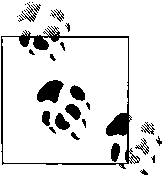
\includegraphics[width=2cm,clip]{paipai.png}
\end{wrapfigure}
\mbox{}\begin{flushleft}在处理EAGAIN时使用一个goto start可能实际上没什么意\\义---你大概只需要不使用非阻塞I/O即可。使用它并不能\\节省时间,相反还引入了更多的循环带来的开销。\end{flushleft} 


\subsection{其他错误码}
其他的错误代码表示编程错误或者(对EIO来说)底层问题。在read()失败后可能的errno值包括: 

\begin{eqlist*}
\item [EBADF]
给出的文件描述符非法,或者不是用可读方式打开的。 
\item [EFAULT]
buf指针不在调用进程的地址空间内。
\item [EINVAL]
文件描述符对应的对象不允许读取。 
\item [EIO]
发生了一个底层I/O错误。
\end{eqlist*}

\subsection{read()大小限制}
size\_t和ssize\_t类型由POSIX确定。size\_t类型用来存储用字节衡量大小的值。ssize\_t类型是有符号的size\_t类型(负值用来表示错误)。在32位系统上,对应的C类型一般分别是unsigned int和int。由于两种类型常常一起使用,ssize\_t的较小范围就潜在地给size\_t的范围作出了限制。

size\_t的最大值为SIZE\_MAX;ssize\_t的最大值为SSIZE\_MAX。如果len比SSIZE\_MAX 大,read()调用的结果是未定义的。在大部分Linux系统上,SSIZE\_MAX是LONG\_MAX,在32位系统上即0x7fffffff。这个数字对一次读入来说已经足够大了,但还是需要记住它。如果你要用前面的读循环代码作为一种通用的读取方式,你可能需要增加如下代码:

\begin{lstlisting}
  if (len > SSIZE_MAX)
      len = SSIZE_MAX;
\end{lstlisting}

一个len为零的read()调用的结果是立即返回且返回值为0。 

\section{用write()来写}

最常见的写文件的系统调用是write()。 write()与read()相对应,也在POSIX.1中定义。 

\begin{lstlisting}
  #include <unistd.h>

  ssize_t write (int fd, const void *buf, size_t count);
\end{lstlisting}

一个write()调用从由文件描述符fd引用文件的当前位置开始,将buf中至多count个字节写入文件中。 不支持定位的文件(像字符设备)总是从“开头”开始写。

成功时,返回写入字节数,并更新文件位置。错误时,返回-1,并将errno设置为相应的值。一个write()可以返回0,但这种返回值没有任何特殊含义;只是表示写入了零个字节。

像read()一样,最基本的用法很简单: 

\begin{lstlisting}
  const char *buf = "My ship is solid!";
  ssize_t nr;
 
  /* write the string in 'buf' to 'fd' */
  nr = write (fd, buf, strlen (buf));
  if (nr == -1)
      /* error */
\end{lstlisting}

与read()仍然相像的是,这种简单用法并不大合适。调用者也需要检查出现部分写的各种可能情况。

\begin{lstlisting}
  unsigned long word = 1720;
  size_t count;
  ssize_t nr;

  count = sizeof (word);
  nr = write (fd, &word, count);
  if (nr == -1)
      /* error, check errno */
  else if (nr != count)
      /* possible error, but 'errno' not set */
\end{lstlisting}

\subsection{部分写}

相对于read()的返回部分读的情况,write()不太可能返回一个部分写的结果。而且,对write()系统调用来说没有EOF情况。对于普通文件,除非发生一个错误,否则write()将保证写入所有的请求,。

那么,对于普通文件,你就不需要进行循环写了。然而对于其他类型——例如套接字——大概得有个循环来保证你真的写入了所有请求的字节。使用循环的另一个好处是,第二次write()调用可能会返回一个错误值用来说明第一次调用为什么进行了一次部分写(尽管这种情况不大常见)。请大家看下面的示例代码:

\begin{lstlisting}
  ssize_t ret, nr;

  while (len != 0 && (ret = write (fd, buf, len)) != 0) {
      if (ret == -1) {
          if (errno == EINTR)
              continue;
          perror ("write");
          break;
      }
      len -= ret;
      buf += ret;
  }
\end{lstlisting}

\subsection{追加模式}

当fd在追加模式下打开时(通过指定O\_APPEND参数),写操作就不从文件描述符的当前位置开始,而是从当前文件末尾开始。

举例来说,假设有两个进程在向同一个文件写。不使用追加模式的话,如果第一个进程向文件末尾写,而第二个进程也这么做,那么第一个进程的文件位置将不再指向文件末尾,而将指向文件末尾减去第二个进程写入的字节数的地方。这意味着多个进程如果不进行显式的同步则不能进行追加写操作,因为它们存在竞争条件。

追加模式避免了这样的问题。它保证文件位置总是指向文件末尾,这样所有的写操作总是追加的,即便有多个写者。你可以认为每个写请求之前的文件位置更新操作是原子操作。文件位置更新至刚刚写入的数据结尾。这和下一个write()调用无关,因为更新文件位置是自动完成的,但可能因为某些奇怪的原因会影响到下一个read()调用。

追加模式在某些任务中很管用,像更新日志文件,但在不少其他方面也没什么用处。

\subsection{非阻塞写}
当fd在非阻塞模式下打开时(通过设置O\_NONBLOCK参数),并且发起的写操作会正常阻塞时,write()系统调用返回-1,并设置errno值为EAGAIN。请求应该在稍后重新发起。通常处理普通文件时不会出现这种事。 

\subsection{其他错误码}
其他值得注意的错误值包括:
\begin{eqlist*}
\item [EBADF]
给定的文件描述符非法,或者不是以写方式打开的。 
\item [EFAULT]
buf指针指向不在进程地址空间内。 
\item [EFBIG]
写操作将使文件大小超过进程的最大文件限制,或者内部实现的限制。 
\item [EINVAL]
给定的文件描述符对应的对象不能用来进行写操作。 
\item [EIO]
发生了一个底层I/O错误。 
\item [ENOSPC]
文件描述符所在的文件系统没有足够的空间。 
\item [EPIPE]
给定文件描述符关联的管道或套接字的读端被关闭。进程也将收到一个SIGPIPE信号。SIGPIPE信号的默认行为是终止收到信号的进程。因而,进程只能在选择忽略,阻塞或者处理该信号时得到这个值。 
\end{eqlist*}

\subsection{write()大小限制}

如果count比SSIZE\_MAX还大,write()调用的结果是未定义的。 count值为零的write()调用将立即返回且返回值为0。 

\subsection{write()的行为}
当一个write()调用返回时,内核已将所提供的缓冲区数据复制到了内核缓冲区中,但却没有保证数据已写到目的文件。write调用返回对于这样的情况来讲确实得太快了。处理器与硬盘的速度差异使这种情况非常明显。

当用户空间应用发起write()系统调用时,Linux内核进行几项检查,然后直接将数据拷贝至一个缓冲区中。稍后,在后台,内核收集所有这样的“脏"缓冲区,将它们排好序,并写入到磁盘上(此过程称为回写)。这使得write调用马上被调用并立刻返回。内核可以将写入操作推迟到空闲阶段,并将很多写操作一起处理。

这种延迟写不会改变POSIX所定义的语义。举例来说,如果一个read调用希望读取刚刚写到缓冲区中但尚未写入磁盘的数据,请求将从缓冲区中响应,而不是读取磁盘上“陈旧”的数据。这种行为实际上提高了效率,因为read只需从内存缓存中读而不用到硬盘中找。读写请求如预计般交错,而结果也如预期那样——当然,前提是在数据写入磁盘前,系统没有崩溃!在这种情况下,即使对于一个应用程序来讲写操作已经成功了,但数据并没有写入到磁盘。

另外一个关于延迟写的问题是对强制写顺序的不可能性。尽管一个应用可能会注意安排它的写请求以使它们将按特定顺序写入磁盘,出于性能方面的考虑,内核将按它觉得合适的顺序重新安排。在系统崩溃时才是问题,而最终所有缓冲区都将正确地写回。尽管如此,绝大多数的应用实际上并不关心写顺序。

最后一个延迟写的问题是关于特定I/O错误的报告。任何在回写中出现的I/O错误——比方说,一个物理磁盘驱动器错误——不会被报告给发起写请求的进程。实际上,缓冲区是和进程完全无关的。多进程可能会更新同一片缓冲区中的数据,而进程可能在数据仍在缓冲区未回写到磁盘前就退出了。另外,你怎么才能在事后与一个写操作失败的进程通讯呢?

内核会尝试将延迟写的风险最小化。为保证数据适时写入,内核创立了一种缓存最大时效机制,并将所有脏的缓存在它们超过给定时效前写入磁盘。用户可以通过/proc/sys/vm/dirty\_expire\_centiseconds来配置这个值。这个值以十毫秒计(百分之一秒)。

强制文件缓存写回也是可以的,甚至可以将所有的写操作同步。这些将是下一节讨论的主题,“同步I/O。”

在本章后面部分,“内核内幕”将深入探讨Linux内核的缓冲回写子系统。 

\section{同步I/O}

尽管同步I/O是一个重要的主题,但不必担心和延迟写相关的问题。由于写缓冲提供了巨大的性能改进,以至于一些半吊子的“现代”系统都用缓冲区实现了延迟写。然而,常有应用想要控制数据被写入磁盘的时间。对于这些需要,Linux内核提供了一些选择来允许用性能换取同步操作。 

\subsection{fsync()和fdatasync()}

最简单的确认数据写入磁盘的方法是使用fsync()系统调用,它在POSIX.1b中定义如下:

\begin{lstlisting}
  #include <unistd.h>

  int fsync (int fd);
\end{lstlisting}

调用fsync()可以保证fd对应文件的脏数据回写到磁盘上。文件描述符fd必须是以写方式打开的。该调用回写数据以及建立的时间戳和inode中的其他属性等元数据。在驱动器确认数据已经全部写入之前不会返回。

在将数据写入硬盘缓存时,fsync()是不可能知道数据是否已经在磁盘上了。磁盘可能报告说数据已写入,但数据可能还在磁盘驱动器的缓存上。幸运的是,在磁盘驱动器缓存中的数据将会很快写入到磁盘。

Linux还提供了fdatasync()系统调用:

\begin{lstlisting}
  #include <unistd.h>

  int fdatasync (int fd);
\end{lstlisting}

这个系统调用完成的事情和fsync()一样,区别在于它仅写入数据。该调用不保证元数据同步到磁盘上,故此可能快一些。一般来说这就够了。

两个函数有相同的用法,非常简单: 

\begin{lstlisting}
  int ret;

  ret = fsync (fd);
  if (ret == -1)
      /* error */
\end{lstlisting}

这两个调用都不保证任何已经更新的包含该文件的目录项同步到磁盘上。这意味着如果文件链接刚刚被更改过,文件数据可能会成功写入磁盘,但却没有关联到相应的目录项上,致使文件不可访问。 为保证任何对目录项的更新也同步到磁盘上,必须对目录本身也调用fsync()进行同步。

\subsection{返回值和错误码}

成功时,两个调用都返回0。失败时,都返回-1,并将errno设置为以下三个值之一:

\begin{eqlist*}
\item [EBADF]
给定的文件描述符不是一个可以写入的合法描述符。 
\item [EINVAL]
给定的文件描述符对应的对象不支持同步。
\item [EIO]
在同步时发生了一个底层I/O错误。这表示一个真正的I/O错误,此类错误经常在错误发生处被捕获。
\end{eqlist*}

一般来讲,即使在相应文件系统上实现了fdatasync()而未实现fsync(),在调用fsync()时也会失败。“偏执”的应用可能会在fsync()返回EINVAL时尝试用fdatasync(),如下所示:

\begin{lstlisting}
  if (fsync (fd) == -1) {
      /*
      * We prefer fsync(), but let's try fdatasync( )
      * if fsync( ) fails, just in case.
      */
      if (errno == EINVAL) {
          if (fdatasync (fd) == -1)
          perror ("fdatasync");
      } else
          perror ("fsync");
  }
\end{lstlisting}

在POSIX标准中fsync()是必要的,而fdatasync()是可选的,因此fsync()在所有常见的、面向普通文件的Linux文件系统都已经实现了。然而,特殊文件类型(可能是那些没有元数据需要同步的文件类型)或者不常见的文件系统或许只实现了fdatasync()。 

\subsection{sync()}

sync()系统调用可以用来对磁盘上的所有缓冲区进行同步,尽管其效率不高,但仍然被广泛使用:

\begin{lstlisting}
  #include <unistd.h>

  void sync (void);
\end{lstlisting}

该函数没有参数,也没有返回值。它总是成功返回,并确保所有的缓冲区——包括数据和元数据——都能写入磁盘。\footnote[1]{好吧,和以往一样,为防止误解在此加以说明:硬盘可能会撒谎,它通知内核缓冲区已经写到磁盘上了,但实际上它们仍在磁盘缓存中。}

标准中并不要求sync()一直等待到所有缓冲区都写到磁盘才返回;只需要调用它来启动将整个将缓冲区写入磁盘的过程即可。由此,一般建议同步多次以确保所有的数据都安全的写入磁盘。然而对于Linux来讲,sync()一定要等到所有的缓冲区都写入才返回。因而,调用一次sync()就够了。

sync()真正派上用场的地方是在工具sync的实现中。应用程序则使用fsync()和fdatasync()将文件描述符指定的数据同步到磁盘。需要注意的是,可能在一个繁忙的系统上sync()操作可能需要几分钟的时间来完成。 

\subsection{O\_SYNC标志}

O\_SYNC标志在open()中使用,使所有在文件上的I/O操作同步。

\begin{lstlisting}
  int fd;

  fd = open (file, O_WRONLY | O_SYNC);
  if (fd == -1) {
      perror ("open");
      return -1;
  }
\end{lstlisting}

读请求总是同步的。如果不同步,将无法保证读取缓冲区中数据的有效性。然而,像先前讨论的那样,write()调用一般是非同步的。调用返回和数据写入磁盘之间没有什么关系。O\_SYNC标志则强制将二者关联,从而保证write()调用进行I/O同步。

O\_SYNC看起来就像是在每个write()操作后都隐式地执行fsync()。尽管这在语法上是毫无问题的,但Linux内核实现的O\_SYNC会更有效一点。

O\_SYNC将在写操作中稍稍影响用户及内核时间(分别为在用户和内核空间消耗的时间)。此外,根据写入文件的大小,可能会使大量的时间消耗在进程的I/O 等待时间(用来等待I/O完成的时间)上,此时的O\_SYNC会使总耗时增加一到两个数量级。这种时间开销增长是非常可观的,所以同步I/O一般是在无计可施情况下的最后选择。

一般情况下,需要确保数据写入磁盘的应用可以使用fsync()或者fdatasync()。因为需要较少的调用(比如,只在某个决定性的操作完成之后),相对于O\_SYNC来讲,开销也更少。 

\subsection{O\_DSYNC和O\_RSYNC}

POSIX为open()定义了另外两个同步相关的标志:O\_DSYNC和O\_RSYNC。在Linux上,这些标志与O\_SYNC同义;它们有相同的行为。


O\_DSYNC标志指定在每次写操作后只有普通数据被同步,元数据则不同步。这看起来就像是在每个写请求后隐式调用fdatasync()一样。因为 O\_SYNC提供了更好的保证,所以没有明确支持O\_DSYNC时并不会导致功能缺失;只是在O\_SYNC有更强要求的情况下有一点性能损失。


O\_RSYNC标志要求读请求像写请求那样进行同步。因此,该标志只能和O\_SYNC或O\_DSYNC一起使用。如前文所述,读操作总是同步的——直到有数据需要返回给用户的时候才会返回。O\_RSYNC标志保证任何读操作的副作用也是同步的。这意味着从一个读操作来更新元数据也须是在调用返回前写入磁盘。实际中,这差不多是要求在read()调用返回前,文件访问时间必须更新到磁盘上的inode中。尽管没有多少意义,Linux还是将O\_RSYNC设定为与O\_SYNC一样(与O\_SYNC和O\_DSYNC的关系不同)。在Linux中通常无法确知O\_RSYNC 的行为;对开发者而言最接近的方式是在每个read()调用后调用fdatasync()。实际上,极少需要这种操作。 

\section{直接I/O}

与其他现代操作系统内核一样,Linux内核实现了一个复杂的缓存、缓冲以及设备和应用之间的I/O管理的层次结构(参见本章末尾“内核内幕”)。一个高性能应用可能希望越过这些复杂的层次结构并进行独立的I/O管理。和I/O系统做斗争实在没什么必要,事实上操作系统层次的工具往往比应用层工具有更好的性能。然而,数据库系统还是倾向于使用他们自己的缓存,以尽可能的减少操作系统的影响。

在open()中使用O\_DIRECT标志会使内核最小化I/O管理的影响。使用该标志时,I/O操作将忽略页缓存机制,直接对用户空间缓冲区和设备进行初始化。所有的I/O将是同步的;操作在完成之前不会返回。

当使用直接I/O时,请求长度,缓冲区对齐,和文件偏移必须是设备扇区大小(通常是512字节)的整数倍。在2.6内核之前,要求更严格:在2.4中,所有的东西都必须对齐到文件系统逻辑块大小(一般是4KB)。为保持兼容性,应用需要对齐到更大的(而且更不便的)逻辑块大小。

\section{关闭文件}

程序完成对某个文件的操作后,可以使用close()系统调用将文件描述符和对应的文件解除关联。

\begin{lstlisting}
  #include <unistd.h>

  int close (int fd);
\end{lstlisting}

close()调用解除了已打开的文件描述符的关联,并分离进程和文件的关联。给定的文件描述符不再有效,内核可以随意将其作为随后的open() 或creat()调用的返回值而重新使用。close()调用在成功时返回0。而错误时返回-1,并设置errno为相应值。用法很简单:

\begin{lstlisting}
  if (close (fd) == -1)
      perror ("close");
\end{lstlisting}

需要注意的是,关闭文件和文件被写入磁盘没什么关系。如果应用想保证文件在关闭前写到磁盘,需要使用一个先前在“同步I/O”中讨论的同步选项。

然而关闭文件的确有些副作用。当最后一个引用某文件的文件描述符关闭后,在内核中表示该文件的数据结构就被释放了。当它释放时,与文件关联的inode的内存拷贝被清除。如果没有什么连接到该inode了,它可能会从内存中清除(也有可能保留在内存中,因为内核为了效率缓存一些inode,但也可能不需要)。如果文件已经从磁盘上解除链接,但在解除前仍保持打开,它在被关闭且inode从内存中移除前就不会真的被删除。因而,对 close()的调用可能会使某个已解除链接的文件最终从磁盘上被删除。

\subsection{错误码}

一个常见的错误是不检查close()的返回值。这样处理可能会忽略了某个重大的错误。某些操作因为延迟的原因,其错误可能在后来才出现,而close()会报告这些错误。

以下是一些在出错时可能出现的errno 值。除了EBADF(给定的文件描述符不合法),最重要的错误值是EIO,这个错误值表明一个可能和实际的close操作并不相关的底层I/O错误。如果忽略出现的错误,文件描述符合法的情况下,总是会被关闭的,并且与其关联的数据结构被释放。

尽管POSIX允许,但close()绝不会返回EINTR。Linux内核开发者们可能很清楚,这样的实现并不明智。

\section{用lseek()查找}

一般的,一个文件中的I/O是线性的,由读写引发的文件位置的隐式更新就是全部需要查找定位的了。然而一些应用需要在文件中跳来跳去。lseek()系统调用能够对给定文件描述符引用的文件位置设定指定值。除了更新文件位置,没有其它的行为,并不初始化任何I/O。 

\begin{lstlisting}
  #include <sys/types.h>
  #include <unistd.h>

  off_t lseek (int fd, off_t pos, int origin);
\end{lstlisting}

lseek()的行为依赖于初始参数,可以为以下值之一:
\begin{eqlist*}
\item [SEEK\_CUR]
当前文件位置fd设置为当前值加上pos,pos可以为负值,零或正值。一个为零的pos返回当前文件位置值。
\item [SEEK\_END]
当前文件位置fd设置为当前文件长度加上pos,pos可以为负值,零或正值。一个为零的pos设置偏移量为文件末尾。
\item [SEEK\_SET]
当前文件位置fd设置为pos。一个为零的pos设置偏移量为文件起始。
\end{eqlist*}

调用在成功时返回新文件位置。错误时返回-1并设置适当的errno值。

举例设置文件位置fd为1825: 

\begin{lstlisting}
  off_t ret;

  ret = lseek (fd, (off_t) 1825, SEEK_SET);
  if (ret == (off_t) -1)
      /* error */
\end{lstlisting}

或者,设置文件位置fd到文件末尾: 

\begin{lstlisting}
  off_t ret;

  ret = lseek (fd, 0, SEEK_END);
  if (ret == (off_t) -1)
      /* error */
\end{lstlisting}

由于lseek()返回更新过的文件位置,可以用SEEK\_CUR和零值来确定文件当前位置:

\begin{lstlisting}
  int pos;

  pos = lseek (fd, 0, SEEK_CUR);
  if (pos == (off_t) -1)
      /* error */
  else
      /* 'pos' is the current position of fd */
\end{lstlisting}

显然,lseek()最常见的用法是来定位一个文件描述符的开始和末尾,或是确定该描述符的当前文件位置。 

\subsection{文件末尾之后进行查找}

lseek()是可以在文件指针超过文件末尾之后进行查找的。举例来说,下面的代码将查找到fd对应的文件末尾之后1688个字节。 

\begin{lstlisting}
  int ret;

  ret = lseek (fd, (off_t) 1688, SEEK_END);
  if (ret == (off_t) -1)
      /* error */
\end{lstlisting}

对这种用法本身来说,查找到文件末尾之后没什么影响——到最新产生的文件位置的读请求会返回EOF。然而如果在接下来对该位置有一个写请求,则会在新旧长度之间建立新的空间,并由零来填充。

这种零填充方式称为“空洞”(hole)。在Unix风格的文件系统上,空洞不占用任何物理上的磁盘空间。这暗示着文件系统上所有文件的大小加起来可以超过磁盘的物理大小。带空洞的文件叫做“稀疏文件”(sparse file)。稀疏文件可以节省可观的空间并提升效率,因为操作那些空洞并不引发任何物理I/O。

一个对文件空洞部分的读请求将返回相应数量的二进制零。 

\subsection{错误码}

出错时,lseek()返回-1,并将errno设置为下面四个之值之一: 

\begin{eqlist*}
\item [EBADF]
给出的文件描述符没有指向任何打开的文件。
\item [EINVAL]
origin的值不是SEEK\_SET,SEEK\_CUR或者SEEK\_END其中之一,或者最终计算的文件位置为负数。事实上,如果出现EINVAL的这两种错误都是很不幸的。前者几乎肯定是一个编译时的错误,而后者可能代表一个隐蔽得多的运行时逻辑错误。
\item [EOVERFLOW]
计算后的文件偏移不能被off\_t表示。这种情况只会发生在32位架构上。当前,文件位置会被修改;而这个错误只是表示不能返回这个值。
\item [ESPIPE]
给出的文件描述符关联到了一个不能执行查找操作的对象上,例如管道,FIFO或套接字。
\end{eqlist*}

\subsection{限制}

文件位置的上限值被限定为off\_t类型的大小。大部分架构定义这个值为C的long类型,在Linux上总是字长(通常是机器通用寄存器的大小)。从内部实现来看,内核将偏移量存储成C的long long类型。这种处理方法在64位机器上没有问题,但在32位机器上作相应查找时可能产生EOVERFLOW错误。 

\section{定位读写}

Linux提供了两种read()和write()的变体来替代lseek(),每个调用都以需要读写的文件位置为参数。完成时,不修改文件位置。

读形式的调用为pread():

\begin{lstlisting}
  #define _XOPEN_SOURCE 500

  #include <unistd.h>

  ssize_t pread (int fd, void *buf, size_t count, off_t pos);
\end{lstlisting}

这个调用从文件描述符fd的pos文件位置读取count个字节到buf中。

写形式的调用为pwrite():

\begin{lstlisting}
  #define _XOPEN_SOURCE 500

  #include <unistd.h>

  ssize_t pwrite (int fd, const void *buf, size_t count, off_t pos);
\end{lstlisting}

这个调用从文件描述符fd的pos文件位置写count个字节到buf中。

除了它们不管当前文件位置,这些调用的行为和read()、wirte()几乎没有区别,它们使用pos提供的值而不是当前位置。此外,在调用完成时,它们不会修改文件位置。换句话说,任何混杂的read()和write()调用可能破坏了定位读写的结果。

两种定位读写调用都只能用于可以进行定位操作的文件描述符。从语义角度来讲,相当于在调用read()或write()前使用 lseek()进行定位,但有仍有三点区别:第一,这些调用更加简单易用,尤其是在文件中做反向移动和随机移动这种技巧性很强的操作时更是如此。第二,当操作完成时,不修改文件位置指针。最后,也是最重要的,避免了任何在使用lseek()时可能出现的潜在竞争。由于线程共享文件描述符,可能在一个线程调用lseek()之后,但尚未进行读写操作前,另一个线程修改文件位置。我们可以通过使用pread()和pwrite()来避免产生这样的竞争。 

\subsection{错误码}

成功时,两个调用返回读或写的字节数。pread()返回零表示EOF;而对pwrite(),一个零值返回表明调用没有写任何东西。出错时,二者均返回-1并设置errno为相应值。对pread()而言,任何对read()或lseek()的errno值都是可能出现的。对pwrite()而言,任何 write()或lseek()的errno值也都是可能出现的。 

\section{截短文件}

Linux提供了两个系统调用来截短文件,二者都在各类POSIX标准中定义并(不同程度的)实现。 它们分别是:

\begin{lstlisting}
  #include <unistd.h>
  #include <sys/types.h>

  int ftruncate (int fd, off_t len);
\end{lstlisting}

和:

\begin{lstlisting}
  #include <unistd.h>
  #include <sys/types.h>

  int truncate (const char *path, off_t len);
\end{lstlisting}

两个系统调用都将文件截短到len指定的长度。ftruncate()系统调用操作一个打开的并且可写的文件描述符fd。truncate()系统调用操作path指定的一个可写文件。二者都在成功时返回0。错误时返回-1,并设置errno为相应值。

这两个系统调用最常见的用途是将文件截短到比原文件长度小一些。成功返回时,文件长度变成len。之前在len和旧长度之间的数据将被忽略,并不可读取。

它们也可以将文件“截短”到比原长度更长,类似于前面“查找到文件末尾之后”中查找加上写操作的结合。扩展出的字节将全部填充为零。

这两个操作均不修改当前文件位置。

举例来看,考虑包含下面内容的74字节大小的文件pirate.txt:

\begin{verbatim}
  Edward Teach was a notorious English pirate.

  He was nicknamed Blackbeard.
\end{verbatim}

从同一个路径下,运行下面的程序: 

\begin{lstlisting}
  #include <unistd.h>
  #include <stdio.h>
  int main( )
  {
      int ret;

      ret = truncate ("./pirate.txt", 45);
      if (ret == -1) {
          perror ("truncate");
          return -1;
      }
      return 0;
  }
\end{lstlisting}

结果产生了包含如下45字节的文件:

\begin{verbatim}
  Edward Teach was a notorious English pirate. 
\end{verbatim}

\section{I/O多路复用}

应用程序常常需要在多于一个文件描述符上阻塞:例如响应键盘输入(stdin)、进程间通信以及同时操作多个文件。基于事件驱动机制的图形用户界面(GUI)应用的主循环中可能包含上百个等待响应的事件。\footnote[1]{主循环对于任何写过GUI应用的人来说是很熟悉的了——像GNOME用一个由GLib,它的基本库提供的主循环。一个主循环允许从一个阻塞点开始监控多个事件并响应。}

在不使用线程,尤其是独立处理每一个文件的情况下,进程无法在多个文件描述符上同时阻塞。如果文件都处于准备好被读写的状态,同时操作多个文件描述符是没有问题的。但一旦在该过程中出现一个未准备好的文件描述符(就是说,如果一个read()被调用,但没有读入数据),则这个进程将会阻塞,不能再操作其他文件。可能阻塞只有几秒钟,但是应用无响应也会造成不好的用户体验。然而,如果该文件描述符始终没有任何可用数据,就可能一直阻塞下去。文件描述符的I/O总是相关的(例如管道),很可能一个文件描述符依赖另外一个文件描述符,直到后者可以被使用前,前者一直处于不可用状态。尤其是对网络应用程序而言,同时打开的多个套接字,会诱发潜在的问题。

试想一下如下场景:当标准输入设备挂起,无数据输出,应用在一个进程间通信相关的文件描述符上阻塞。应用只有在阻塞的IPC文件描述符返回数据后,才能确知键盘输入已经挂起。如果被阻塞的操作没有返回,情况又会怎样呢?

如前所述,非阻塞I/O 可以作为这个问题的一个解决方案。使用非阻塞I/O,应用可以发起I/O请求并返回一个特别的错误,从而避免阻塞。从两个方面来讲,这种方法效率较差。首先,进程需要以某种不确定的方式不断发起I/O操作,直到某个打开的文件描述符准备好进行I/O。这种设计很糟糕。其次,如果程序可以睡眠的话将更加有效,可以让处理器进行其他工作,直到一个或更多文件描述符可以进行I/O时再唤醒。

进入I/O多路复用。

I/O多路复用允许应用在多个文件描述符上同时阻塞,并在其中某个可以读写时收到通知。这时I/O多路复用就成了应用的关键所在,一般来讲I/O多路复用的设计遵循以下原则: 

\begin{enumerate}
\item I/O多路复用:当任何文件描述符准备好I/O时告诉我
\item 在一个或更多文件描述符就绪前始终处于睡眠状态。
\item 唤醒:哪个准备好了?
\item 在不阻塞的情况下处理所有I/O就绪的文件描述符。
\item 返回第一步,重新开始。 
\end{enumerate}

Linux提供了三种I/O多路复用方案:select,poll和epoll。我们先看看前两个,我们将在第四章讨论最后一个,那是Linux特有的高级方法。 

\subsection{select()}

select()系统调用提供了一种实现同步I/O多路复用的机制: 

\begin{lstlisting}
  #include <sys/time.h>
  #include <sys/types.h>
  #include <unistd.h>

  int select (int n,
 	      fd_set *readfds,
	      fd_set *writefds,
	      fd_set *exceptfds,
	      struct timeval *timeout);
  FD_CLR(int fd, fd_set *set);
  FD_ISSET(int fd, fd_set *set);
  FD_SET(int fd, fd_set *set);
  FD_ZERO(fd_set *set);
\end{lstlisting}

在指定的文件描述符准备好I/O之前或者超过一定的时间限制,select()调用就会阻塞。

监测的文件描述符可以分为三类,分别等待不同的事件。监测readfds集合中的文件描述符,确认其中是否有可读数据(也就是说,读操作可以无阻塞的完成)。监测writefds集合中的文件描述符,确认其中是否有一个写操作可以不阻塞地完成。监测exceptefds中的文件描述符,确认其中是否有出现异常发生或者出现带外(out-of-band)数据(这种情况只适用于套接字)。指定的集合可能为空(NULL),相应的,select()则不对此类时间进行监视。

成功返回时,每个集合只包含对应类型的I/O就绪的文件描述符。举例来说,readfds集合中有两个文件描述符:7和9。当调用返回时,如果7还在集合中,该文件描述符就准备好进行无阻塞I/O了。如果9已不在集合中,它可能在被读取时会发生阻塞。(我这里说“可能”是因为数据可能在调用完成后已经就绪了。在这种情况下,下一个select()调用返回时,将该文件描述符返是就绪的。\footnote[1]{这是因为select()和poll()都是电平触发而不是边沿触发的。将在第四章讨论的epoll(),可以在任一种方式下工作。边沿触发操作简单一些,但允许在未注意时错过I/O事件。})

第一个参数n,等于所有集合中文件描述符的最大值加一。这样,select()的调用者需要找到最大的文件描述符值,并将其加一后传给第一个参数。

timeout参数是一个指向timeval结构体的指针,定义如下: 

\begin{lstlisting}
 #include <sys/time.h>

 struct timeval {
	long tv_sec; /* seconds */
	long tv_usec; /* microseconds */
 };
\end{lstlisting}

如果这个参数不是NULL,即使此时没有文件描述符处于I/O就绪状态,select()调用也将在tv\_sec秒tv\_usec微秒后返回。返回时,这个结构体的状态在大多俗话Unix系统中都是未定义的。这样的话,每次调用前都必须重新初始化(还有集合中的文件描述符)。较新版本的Linux会自动将该值改为剩余的时间。这样,如果时限是5秒,在某个文件描述符准备好时过去了3秒,tv.tv\_sec在返回时就还是2。

如果时限中的两个值都是零,调用会立即返回,并报告调用时所有事件对应的文件描述符均不可用,且不等待任何后续事件。

集合中的文件操作符并不直接操作,而是通过辅助宏来进行管理。这就允许Unix系统按其所希望的方式来实现,大多数系统,将其实现为位数组。FD\_ZERO从指定集合中移除所有文件描述符。在每次使用select()之前,需要调用该宏。 

\begin{lstlisting}
  fd_set writefds;
 
  FD_ZERO(&writefds);
\end{lstlisting}

FD\_SET向指定集合中添加一个文件描述符,而FD\_CLR从指定集合中移除一个文件描述符。 

\begin{lstlisting}
  FD_SET(fd, &writefds); /* add 'fd' to the set */
  FD_CLR(fd, &writefds); /* oops, remove 'fd' from the set */
\end{lstlisting}

设计良好的代码应该从不使用FD\_CLR。一般来讲,很少使用该宏。

FD\_ISSET测试一个文件描述符在不在给定集合中。如果在,则返回一个非零值,否则用0表示不在。一般在select()调用返回后使用FD\_ISSET来检查一个文件描述符是否就绪。 

\begin{lstlisting}
  if (FD_ISSET(fd, &readfds))
      /* 'fd' is readable without blocking! */
\end{lstlisting}

由于文件描述符集合是静态建立的,所以对于文件描述符数量的上限和文件描述符的最大值均有限制,二者都由FD\_SETSIZE设定。在Linux上,这个值是1024。我们将在本章稍后来看看这个限制的作用。 

\subsection{返回值和错误码}

成功时,select()返回在所有三个集合中I/O就绪的文件描述符的数目。如果给出了时限,返回值可能为0。错误时返回-1,而且errno被设置为下列值之一: 

\begin{eqlist*}
\item [EBADF]
某一个集合中的一个文件描述符非法。
\item [EINTR]
等待时捕获了一个信号,可以重新发起调用。
\item [EINVAL]
参数n是负数,或者给出的时限不合法。
\item [ENOMEM]
没有足够的内存完成请求。
\end{eqlist*}

\subsubsection{select()示例程序}

我们来看看下面的样例程序,虽然简单但是对select()用法的介绍却非常完整。这个例子中,等待stdin的输入的阻塞时限设置为5秒钟。由于只监测了一个文件描述符,实际上这不是I/O多路复用,但系统调用的用法却很清晰。 

\begin{lstlisting}
  #include <stdio.h>
  #include <sys/time.h>
  #include <sys/types.h>
  #include <unistd.h>

  #define TIMEOUT 5 /* select timeout in seconds */
  #define BUF_LEN 1024 /* read buffer in bytes */

  int main (void)
  {
      struct timeval tv;
      fd_set readfds;
      int ret;
      /* Wait on stdin for input. */
      FD_ZERO(&readfds);
      FD_SET(STDIN_FILENO, &readfds);
      /* Wait up to five seconds. */
      tv.tv_sec = TIMEOUT;
      tv.tv_usec = 0;
      /* All right, now block! */
      ret = select (STDIN_FILENO + 1,
		    &readfds,
		    NULL,
		    NULL,
		    &tv);
      if (ret == -1) {
          perror ("select");
          return 1;
      } else if (!ret) {
          printf ("%d seconds elapsed.\n", TIMEOUT);
          return 0;
      }

      /*
       * Is our file descriptor ready to read?
       * (It must be, as it was the only fd that
       * we provided and the call returned
       * nonzero, but we will humor ourselves.)
       */
      if (FD_ISSET(STDIN_FILENO, &readfds)) {
          char buf[BUF_LEN+1];
	  int len;
	  /* guaranteed to not block */
	  len = read (STDIN_FILENO, buf, BUF_LEN);
	  if (len == -1) {
	      perror ("read");
	      return 1;
	  }
	  if (len) {
	      buf[len] = '\0';
	      printf ("read: %s\n", buf);
          }
          return 0;
      }

      fprintf (stderr, "This should not happen!\n");
      return 1;
  }
\end{lstlisting}

\subsubsection{用select()实现可移植的sleep()}

由于select()在各种Unix系统中都很容易实现,相对于微秒级精度的睡眠机制来讲,经常将select()做为一种可移植的微秒级的睡眠机制。该方法通过将三个集合值设为空(NULL),将超时值设置为非空(non-NULL)来实现。 

\begin{lstlisting}
  struct timeval tv;

  tv.tv_sec = 0;
  tv.tv_usec = 500;

  /* sleep for 500 microseconds */
  select (0, NULL, NULL, NULL, &tv);
\end{lstlisting}

当然,Linux提供了高精度的睡眠机制的实现,具体内容,我们将在第十章中学习。

\subsubsection{pselect()}

在4.2BSD中首次引入的select()很受欢迎,但POSIX定义了自己的方法——pselect(),在POSIX 1003.1g-2000和后来的POSIX 1003.1-2001中对pselect()做了如下定义: 

\begin{lstlisting}
  #define _XOPEN_SOURCE 600
  #include <sys/select.h>

  int pselect (int n,
      fd_set *readfds,
      fd_set *writefds,
      fd_set *exceptfds,
      const struct timespec *timeout,
      const sigset_t *sigmask);

  FD_CLR(int fd, fd_set *set);
  FD_ISSET(int fd, fd_set *set);
  FD_SET(int fd, fd_set *set);
  FD_ZERO(fd_set *set);
\end{lstlisting}

pselect()和select()有三点不同:

1. pselect()的timeout参数使用了timespec结构,而不是timeval结构。timespec使用秒和纳秒,不是秒和毫秒,从理论上来讲更精确一些。实际上,两者在毫秒精度上已经都不可靠了。

2. pselect()调用并不修改timeout参数。这个参数在后续调用时也不需要重新初始化。

3. select()调用没有sigmask参数。当这个参数被设置为零时,pselect()的行为等同于select()。

timespec结构体定义为如下形式: 

\begin{lstlisting}
  #include <sys/time.h>

  struct timespec {
      long tv_sec; /* seconds */
      long tv_nsec; /* nanoseconds */
  };
\end{lstlisting}

添加pselect()到Unix工具箱的主要原因是为了增加sigmask参数,以此来解决信号和等待文件描述符之间的竞争条件(信号在第九章深入讨论)。假设一个信号处理程序设置了一个全局标记(大部分信号处理程序都这么干),进程在每次调用select()前都要检查这个标记。现在,假如在检查标记和调用之间接收到信号,应用可能会阻塞,并不再响应该信号。pselect()提供了一组可阻塞的信号,可以解决这个问题。阻塞的信号直到解除阻塞才会被处理。一旦pselect()返回,内核就恢复旧的信号掩码。详见第九章。

2.6.16内核之前,Linux实现的pselect()还不是一个系统调用,而是由glibc提供的一个简单的对select()的封装。该方法使竞争条件出现的风险最小化,但是没有根本消除。当真正引入一个系统调用,才彻底解决竞争问题。

如果不考虑pselect()中(相对不大的)改进,大多数应用会继续使用select(),部分是出于习惯,其他则是考虑可移植性。

\subsection{poll()}

poll()系统调用是System V的I/O多路复用解决方案。它解决了一些select()的不足,不过select()仍经常被使用(还是出于习惯和可移植性的考虑):

\begin{lstlisting}
  #include <sys/poll.h>

  int poll (struct pollfd *fds, unsigned int nfds, int timeout);
\end{lstlisting}

与select()使用的三个基于位掩码的文件描述符集合不同,poll()使用一个简单的nfds个pollfd结构体构成的数组,fds指向该数组。结构体定义如下:

\begin{lstlisting}
  #include <sys/poll.h>

  struct pollfd {
      int fd; /* file descriptor */
      short events; /* requested events to watch */
      short revents; /* returned events witnessed */
  };
\end{lstlisting}

每个pollfd结构体指定监视单一的文件描述符。可以传递多个结构体,使得poll()监视多个文件描述符。每个结构体的events字段是要监视的文件描述符事件的一组位掩码。用户设置这个字段。revents字段则是发生在该文件描述符上的事件的位掩码。内核在返回时设置这个字段。所有在 events字段请求的事件都可能在revents字段中返回。下面是合法的事件: 

\begin{eqlist*}
\item [POLLIN]
有数据可读。 
\item [POLLRDNORM]
有正常数据可读。
\item [POLLRDBAND]
有优先数据可读。
\item [POLLPRI]
有高优先级数据可读。
\item [POLLOUT]
写操作不会阻塞。
\item [POLLWRNORM]
写正常数据不会阻塞。
\item [POLLBAND]
写优先数据不会阻塞。
\item [POLLMSG]
有一个SIGPOLL消息可用。
\end{eqlist*}

另外,如下事件可能在revents中返回: 

\begin{eqlist*}
\item [POLLER]
给出文件描述符上有错误。
\item [POLLHUP]
文件描述符上有挂起事件。
\item [POLLNVAL]
给出的文件描述符非法。
\end{eqlist*}

这些在events中没有意义,而总是在合适时返回。使用poll(),不像select()那样,你无需另外请求报告异常。 

POLLIN | POLLPRI等价于select()的读事件,而POLLOUT | POLLWRBAND等价于select()的写事件。POLLIN等价于POLLRDNORM | POLLRDBAND,而POLLOUT等价于POLLWRNORM。

举例来说,监视一个文件描述符是否可读写,我们需设置events为POLLIN | POLLOUT。返回时,我们将在revents中是否有相应的标志。如果设置了POLLIN,文件描述符就需要能非阻塞读。如果设置了POLLOUT,文件描述符需要能非阻塞写。这些标志并不相互排斥:二者都可以设置,表示可以在文件描述符上读写,并都不会阻塞。

timeout参数指定在任何I/O就绪前需要等待时间的长度,以毫秒计。负值表示永远等待。一个零值表示调用立即返回,列出所有未准备好的I/O,但不等带任何其他事件。这种情况下,poll()就如同其名,轮询一次后立即返回。 

\subsubsection{返回值和错误码}

成功时,poll()返回具有非零revents字段的文件描述符个数。超时前没有任何事件发生则返回零。失败时返回-1,errno被设置为下列值之一: 

\begin{eqlist*}
\item [EBADF]
一个或更多结构体中有非法的文件描述符。
\item [EFAULT]
指向fds的指针超出了进程地址空间。 
\item [EINTR]
在请求事件发生前收到了一个信号,可以重新调用。
\item [EINVAL]
nfds参数超过了RLIMIT\_NOFILE值。 
\item [ENOMEM]
没有足够的内存完成请求。
\end{eqlist*}

\subsubsection{poll()的例子}

我们来看一个使用poll()的样例程序,要同时检测一个stdin读和一个stdout写是否阻塞: 

\begin{lstlisting}
  #include <stdio.h>
  #include <unistd.h>
  #include <sys/poll.h>

  #define TIMEOUT 5 /* poll timeout, in seconds */

  int main (void)
  {
      struct pollfd fds[2];
      int ret;

      /* watch stdin for input */
      fds[0].fd = STDIN_FILENO;
      fds[0].events = POLLIN;
      /* watch stdout for ability to write (almost always true) */
      fds[1].fd = STDOUT_FILENO;
      fds[1].events = POLLOUT;

      /* All set, block! */
      ret = poll (fds, 2, TIMEOUT * 1000);
      if (ret == -1) {
          perror ("poll");
          return 1;
      }

      if (!ret) {
          printf ("%d seconds elapsed.\n", TIMEOUT);
          return 0;
      }

      if (fds[0].revents & POLLIN)
          printf ("stdin is readable\n");

      if (fds[1].revents & POLLOUT)
          printf ("stdout is writable\n");

      return 0;
  }
\end{lstlisting}

运行,我们得到了预期的结果:

\begin{verbatim}
  $ ./poll

  stdout is writable
\end{verbatim}

再次运行,但将一个文件重定向到标准输入,我们看到了两个事件:

\begin{verbatim}
  $ ./poll < ode_to_my_parrot.txt

  stdin is readable

  stdout is writable
\end{verbatim}

假设我们在一个应用中使用了poll(),我们无需在每次调用时重新构建pollfd结构体。相同的结构可能会被反复传递;必要时内核会把revents字段清空。 

\subsubsection{ppoll()}

Linux提供了一个poll()的近似调用——ppoll()。ppoll()和pselect()同源,然而和pselect()不同的是,ppoll()是Linux的专有调用:

\begin{lstlisting}
  #define _GNU_SOURCE
  #include <sys/poll.h>

  int ppoll (struct pollfd *fds,
             nfds_t nfds,
	     const struct timespec *timeout,
	     const sigset_t *sigmask);
\end{lstlisting}

像pselect()那样,timeout参数以秒和纳秒计指定了时限,而sigmask参数提供了一组等待处理的信号。 

\subsection{poll()与select()}

尽管它们完成一样的工作,但poll()系统调用仍然优于select(): 

\begin{itemize}
\item \begin{flushleft}poll()无需使用者计算最大的文件描述符值加一和传递该参数。\end{flushleft}
\item \begin{flushleft}poll()在应对较大值的文件描述符时更具效率。想像一下用select()监视值为900的文件描述符——内核需要检查每个集合中的每个比特位,直到第九百个。\end{flushleft}
\item \begin{flushleft}select()的文件描述符集合是静态大小的,所以要作出权衡:要么集合很小,限制了select()可以监视的文件描述符的最大值,要么较大,但是效率不高。尤其是当不能确定集合的组成是否稀疏时,对较大位掩码的操作效率不高。\footnote[1]{如果位掩码是稀疏组成的,每个带有掩码的字都可以用零来检测;只在操作返回失败值时需要对每个位进行检测。然而这项工作很浪费,如果位掩码比较稠密的话。}使用poll()则可以创建合适大小的数组。只需要监视一项或仅仅传递一个结构体。\end{flushleft}
\item \begin{flushleft}若用select(),文件描述符集合会在返回时重新创建,这样的话之后每个调用都必须重新初始化它们。poll()系统调用分离了输入(events字段)和输出(revents字段),数组无需改变即而重用。\end{flushleft}
\item \begin{flushleft}select()的timeout参数在返回时是未定义的。可移植的代码需要重新初始化它。然而pselect()没有这个问题。\end{flushleft}
\end{itemize}

但是select()系统调用的确有几个不错的地方:

\begin{itemize}
\item \begin{flushleft}poll()由于某些Unix系统不支持poll(),所以select()的可移植性更好。\end{flushleft}
\item \begin{flushleft}select()提供了更好的超时方案:直到微秒级。ppoll()和pselect()在理论上都提供纳秒级的精度,但在实际中,没有任何调用可以可靠的提供哪怕是微秒级的精度。\end{flushleft}
\end{itemize}

比poll()和select()更好的是epoll接口,一个Linux特有的I/O多路复用解决方案,我们将在第四章探讨。

\section{内核内幕}

这部分来看看Linux内核是如何实现I/O的,集中关注三个主要的内核子系统:虚拟文件系统(VFS),页缓存,和页回写。这些子系统使Linux中的I/O看起来无缝运转,且更加高效。 

\begin{wrapfigure}{l}{2.5cm}
  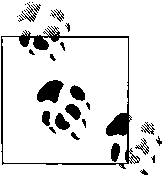
\includegraphics[width=2cm,clip]{paipai.png}
\end{wrapfigure}
\mbox{}在第四章,我们将看到第四个子系统,I/O调度器。 

\subsection{虚拟文件系统}

虚拟文件系统(有时也叫做virtual file switch)是一种Linux内核的文件操作的抽象机制。它允许内核在无需了解文件系统类型的情况下,使用文件系统函数和操作文件系统数据。

VFS实现这种抽象的方法是使用一种通用文件模型(common file model),它是所有Linux文件系统的基础。基于函数指针和各种面向对象方法\footnote[1]{是的,在C中。},通用文件模型提供了一种Linux内核文件系统必须遵循的框架。它允许VFS对文件系统发起请求。框架提供了钩子来支持读,建立链接,同步以及其他功能。每种文件系统再使用合适的函数来处理相应操作。

这种方法强制要求文件系统间需要有一定的共性。举个例子,VFS工作于inode,superblock和目录条目之上。一个非Unix 的文件系统可能缺少类Unix的概念如inodes,只不过需要去处理解决。确实如此:Linux可以很好的支持像FAT和NTFS这样的文件系统。

VFS的好处太多了。一个简单的系统调用可以从任意媒介上的任意文件系统上读;一个简单的工具可以从一个文件系统拷贝到另一个上。所有文件系统都支持同样的概念,同样的接口,和同样的调用。一切都正常工作——而且工作得很好。

当一个应用发起一个read()系统调用,就开始了一段奇妙的旅程。C库提供了系统调用的定义,而在编译器调用转化为适当的陷阱态。当一个用户空间进程转入内核态,则转交系统调用处理器处理,最终交给read()系统调用,内核确认文件描述符所对应的对象类型。然后内核调用与相关类型对应的 read()函数。对于文件系统而言,这个函数是文件系统代码的一部分。然后该函数继续其工作——举例来说,从文件系统中读取数据——并把数据返回给用户空间的read()调用,该调用返回复制数据到用户空间的系统调用处理器,然后将数据复制到用户空间,最后read()系统调用返回而进程继续执行。

对系统程序员来说,VFS的影响是很重要的。程序员不需担心文件所在的文件系统或者介质。通用系统调用——read(),write(),以及其他——能够在任意支持的文件系统和介质上操作文件。 

\subsection{页缓存}

页缓存是一种在内存中保存最近在磁盘文件系统上访问过的数据的方式。相对于现在的处理器速度而言,磁盘访问速度过慢。在内存中保存被请求数据,内核在接下来对相同数据的后续请求可以直接从内存中读取,尽量避免重复磁盘访问。

页缓存利用了引用局部性(locality of reference)的一种方法——时间局部性(temporal locality),该方法使刚被访问资源很可能会在不久后再次被访问。由于避免了费时的磁盘访问,内存在第一次访问时缓存数据的开销因而得到补偿

页缓存是内核寻找文件系统数据的第一目的地。只有缓存中找不到时内核才会调用存储子系统从磁盘中读取数据。当数据第一次读取后,就会从磁盘读入页缓存中,并从缓存中返回给应用。如果那项数据被再次读取,就直接从缓存中返回。通过页缓存的所有操作执行都是透明的,保证它的数据总是相关且有效的。

Linux页缓存大小是动态的。随着I/O操作将越来越多的数据带入内存,页缓存也随之增大,消耗掉空闲的内存。如果页缓存最终确实消耗掉了所有的空闲内存,而且有新增的存储要求出现,页缓存就会被削减,释放它最少使用的页,将空间让给“真正的”内存使用。这种处理是自动进行的。一个动态变化的缓存允许Linux使用所有的系统内存,并缓存尽可能多的数据。

向磁盘交换一块很少使用的数据,比从页缓存中清除掉一条常常使用的且很可能将在下次重读中使用的数据更有意义(交换允许内核在磁盘上存储数据,得到比机器的RAM更大的内存空间)。Linux内核实现了一些平衡交换数据和清理页缓存(以及其他驻存项目)的启发式方法。这些启发式方法可能会决定用交换数据到磁盘来代替清理页缓存,尤其是在交换的数据并未使用时。

交换和缓存间的平衡可以通过 /proc/sys/vm/swappiness 来调整。这个文件可以在0到100间取值,默认为60。较高的值表示倾向于在内存中保留页缓存,较低的值表示更倾向于清理页缓存而不是进行交换。

引用局部性(locality of reference)的另一种形式是空间局部性(sequential locality),是关于数据的连续使用的性质。基于这个原理,内核实现了页缓存预读技术。预读是在每次读请求时从磁盘数据中读取更多的数据到页缓存中的动作——多读一点点会很有效。当内核从磁盘读取一块数据时,也会读取接下来一两块数据。一次读取较大的连续数据块时磁盘不需要经常寻道,所以会比较有效,。另外,内核可以在进程操作第一块读取数据时完成预读。像经常发生的那样,如果进程继续对接下来的块提交一个新的读请求,内核就可以不用发起磁盘 I/O而直接将预读数据转交。

和页缓存类似,内核管理预读也是动态的。如果它注意到一个进程持续使用预读来的数据,内核就会增加预读窗口,因而预读进更多的数据。预读窗口最小为16KB,最大128KB。反之,如果内核发现预读没有造成任何有用的命中——就是说,应用在文件中来回查找而不是连续的读——它可以完全关闭预读。

页缓存的存在对程序员来讲是透明的。系统程序员一般来说不需要优化代码以期从页缓存机制中得到更多好处(除非是在用户空间实现这样一种缓存)。一般的,有效率的代码就是以最大限度利用页缓存。另一方面,利用预读也不错。虽然不总是如此,但多数情况下连续文件I/O通常多于随机访问。 

\subsection{页回写}

像先前在“write()的行为”中讨论的那样,内核使用缓冲区来延迟写操作。当一个进程发起写请求,数据被拷贝进一个缓冲区,并将该该缓冲区标记为" 脏"的,这意味着内存中的拷贝要比磁盘上的新。此时,写请求就可以返回了。如果对同一个数据块有新的写请求,缓冲区就更新为新数据。在该文件其他部分的写请求则开辟新的缓冲区。 

最终那些"脏"缓冲区需要写入磁盘,将磁盘文件和内存数据同步。这就是所谓的回写。以下两个条件会触发回写: 

\begin{itemize}
\item \begin{flushleft}当空闲内存小于设定的阈值时,脏的缓冲区就会回写到磁盘上,被清理的缓冲区可能会被移除,来释放内存空间。\end{flushleft}
\item \begin{flushleft}当一个脏的缓冲区寿命超过设定的阈值时,缓冲区被回写至磁盘。以此来避免数据的不确定性。 \end{flushleft}
\end{itemize}

回写由一些叫做pdflush的内核线程操作(推测可能是page dirty flush之意,但谁知道呢)。当以上两种情况之一出现时,pdflush线程被唤醒,并开始将脏的缓冲区提交到磁盘,直到没有触发条件被满足。

可能同时有多个pdflush线程在回写。这么做是为了更好的利用并行性而避免拥塞。拥塞避免机制确保在等待向某个块设备进行写操作时,其他的写操作不被积压下来。如果来自其他块设备有脏缓冲区存在,其他pdflush线程就会充分利用每一块设备。这改良了以前内核的一处不足:先前的pdflush线程(bdflush,一个单一线程)可能要消耗掉所有的时间来等待一个块设备,而同时其他块设备处于空闲。在一台现代机器上,Linux内核现在可以使许多个磁盘维持饱和状态。

缓冲区在内核中使用buffer\_head结构来表示。这个数据结构跟踪各种各样与缓冲区关联的元数据,例如缓冲区是干净的还是脏的。同时,它也维护了一个指向实际数据的指针。这部分数据保存在页缓存中。用这样的方式,将缓冲子系统和页缓存统一了起来。

在早期Linux内核版本中——2.4之前——缓冲子系统与页缓存是分离的,这样就同时有一个页缓存和一个缓冲缓存。这意味着数据可以同时在缓冲缓存(作为脏的缓冲区)和页缓存(用来缓存数据)之中存在。自然的,同步这两块缓存要用一些时间。在2.4 Linux内核中引入的统一的页缓存,这是一个不错的改进。

Linux中的延迟写和缓冲子系统可以使写操作迅速完成,代价是要冒着在电源故障时出现数据丢失的风险。为避免这种风险,关键性应用可以使用同步I/O(在本章先前讨论过)。 

\section{结论}

这一章讨论了Linux系统编程的基础:文件I/O。在Linux这样一个一切皆文件的操作系统中,知道如何打开,读,写和关闭文件是非常重要的。所有这些操作都是传统的Unix方式,在多种标准中都有谈及。

下一章集中处理缓冲I/O,以及标准C库的标准I/O接口。标准C库不仅仅是出于方便考虑;用户空间的缓冲I/O提供了关键的性能提升。 


